\documentclass[11pt,a4paper]{article}

% --- Core Packages ---
\usepackage[utf8]{inputenc}
\usepackage[T1]{fontenc}
\usepackage[expansion=false]{microtype}
\usepackage{amsmath,amssymb,amsfonts}
\usepackage{graphicx}
\graphicspath{{figures/}{./}}
\usepackage{booktabs}
\usepackage{tabularx}
\usepackage{siunitx}
\usepackage{xcolor}
\usepackage{tcolorbox}
\usepackage{caption}
\usepackage{subcaption}
\usepackage{geometry}
\usepackage{hyperref}
\usepackage{lmodern}

% --- Page Geometry ---
\geometry{
    a4paper,
    top=1.0in,
    bottom=1.0in,
    left=1.05in,
    right=1.05in,
    headheight=14pt,
    footskip=28pt
}
\linespread{1.06}

% --- Color Definitions ---
\definecolor{nasaBlue}{RGB}{11, 61, 145}
\definecolor{marsRed}{RGB}{185, 55, 35}
\definecolor{deepSlate}{RGB}{30, 41, 59}
\definecolor{sandRule}{RGB}{200, 190, 175}
\definecolor{boxBg}{RGB}{248, 249, 250}
\definecolor{boxBorder}{RGB}{220, 225, 230}

% --- Hyperref Setup ---
\hypersetup{
    colorlinks=true,
    linkcolor=nasaBlue,
    citecolor=nasaBlue,
    urlcolor=nasaBlue,
    pdfauthor={Justin Bogner},
    pdftitle={Quantitative Morphometry and Perspective Geometry of an Anomalous Cylindrical Feature in Curiosity Mastcam Imagery}
}

% --- Custom Callout Box ---
\newtcolorbox{summarybox}[1][]{
    colback=boxBg,
    colframe=nasaBlue,
    fonttitle=\bfseries\sffamily,
    coltitle=white,
    boxrule=1pt,
    arc=4pt,
    left=10pt,
    right=10pt,
    top=8pt,
    bottom=8pt,
    title=#1
}

% --- Helper Macros ---
\newcommand{\pdsframe}{\texttt{3556MR}\allowbreak\texttt{102517}\allowbreak\texttt{0721700585C00\_DXXX}}

% --- Document Metadata ---
\title{\vspace{-1.5cm}\textbf{\Large Quantitative Morphometry and Perspective Geometry of an Anomalous Cylindrical Feature in Curiosity Mastcam Imagery}\\[0.25cm]\large\textsf{Sol 3556 Observation in Paraitepuy Pass, Gale Crater, Mars}}
\author{\textbf{Justin Bogner}}
\date{October 2026}

\begin{document}

\maketitle

\begin{abstract}
\noindent High-resolution surface imaging acquired by the Mars Science Laboratory (\textit{Curiosity}) rover on Sol 3556 in Paraitepuy Pass, Mount Sharp (Gale Crater), reveals a geometrically regular, highly anomalous cylindrical structure resting upon the Martian regolith. Using the raw Planetary Data System (PDS4) archive for Mastcam Right-eye context imaging (frame \pdsframe), we integrate the flight-calibrated CAHVOR camera model, Remote Sensing Mast (RSM) kinematic telemetry, and the rover attitude quaternion in the gravity-aligned local Site Frame. This resolves prior empirical standoff uncertainties, narrowing absolute physical scale variance from $\pm 10\text{--}15\%$ down to $\pm 2.3\%$. The object is situated in the immediate foreground at a true slant range of $d = 5.17 \pm 0.12\,\text{m}$ ($0.3865\,\text{mm / native pixel}$). Fitting an unconstrained conic to the front rim establishes an ellipse with major axis $2a = 51.92\,\text{px}$ in the high-resolution crop ($40.0\,\text{px}$ on the native sensor), resolving an outer cylinder diameter $D = 15.5 \pm 0.4\,\text{mm}$ ($1.55\,\text{cm}$). Affine de-projection confirms that this ellipse resolves to a mathematically true Euclidean circle with radius $R_1 = 26.91\,\text{px}$ ($\sigma_r = 0.74\,\text{px}$, $\pm 1.4\%$ radial residual). At the rear of the structure, sub-pixel gradient optimization localizes a coherent curved terminus with apparent radius $R_2 = 10.20\,\text{px}$ ($37.9\%$ of the front rim). Under central perspective projection ($R \propto 1/Z$), this scaling establishes that the far end recedes into scene depth by a factor of $Z_{\text{rear}} / Z_{\text{front}} \approx 2.64$. The central longitudinal axis ($L_{\text{proj}} = 77.4\,\text{px}$, $\theta = 41.9^\circ$, physical visible projection $22.0 \pm 0.5\,\text{mm}$) and the common external flank tangents enclose the sunlit hull with sub-pixel fidelity, resolving a true 3D cylinder length of $L_{\text{3D}} = 47.1 \pm 1.1\,\text{mm}$ ($4.71\,\text{cm}$) with a length-to-diameter aspect ratio of $L_{\text{3D}} / D \approx 3.0$. Furthermore, empirical delineation of the ground contact line ($y = -0.410\,x + 201.50$, $-22.3^\circ$) establishes that the upper $68.8\%$ of the circular front face and the full longitudinal sunlit flank remain exposed to the sky, while the lower $31.2\%$ circular sector (the dashed cyan arc below the regolith line) is submerged beneath the sediment. Finally, high-noon solar shadow geometry (Sun elevation $69.82^\circ$, local solar noon Sol 3556 12:10:14) independently cross-validates vertical relief and surface contact. We evaluate candidate hypotheses: natural geologic ventifaction, miniature terrestrial aerospace hardware debris (e.g., pyro-actuator casings or drill sleeves), and the open possibility of an artificial artifact of unknown provenance.
\end{abstract}

\vspace{0.3cm}
\noindent\textbf{Keywords:} Mars Science Laboratory, Curiosity Rover, Mastcam, CAHVOR Model, PDS4 Telemetry, Projective Geometry, Photometry, Planetary Forensics.

\vspace{0.3cm}
\noindent\textcolor{sandRule}{\rule{\textwidth}{0.6pt}}
\vspace{0.3cm}

\section{Introduction and Observational Context}

During traverse operations on Sol 3556 (August 7, 2022), NASA's Mars Science Laboratory (\textit{Curiosity}) rover documented the layered sulfate-bearing strata of Paraitepuy Pass, located on the northern slopes of Mount Sharp (Aeolis Mons) within Gale Crater ($4.59^\circ\text{S}, 137.44^\circ\text{E}$). Routine context imaging by the Mast Camera (Mastcam) Right-eye instrument (focal length $f = 100\,\text{mm}$, instantaneous field of view $\text{IFOV} = 0.074\,\text{mrad/pixel}$) captured frame \pdsframe.

Embedded within the local sand and pebble regolith is a conspicuous, highly regular object whose geometric linearity and smooth albedo stand in stark contrast to the surrounding fractured, heterogeneous sedimentary rocks. The anomaly was first identified in raw Planetary Data System archives by independent analyst Rami Bar Ilan in August 2022. It subsequently drew commentary from Harvard astrophysicist Avi Loeb \cite{loeb2022}, who noted the object's smooth, unweathered cylindrical geometry and planar circular face, visually estimating its length as $\approx 20\text{--}30\,\text{cm}$ under an uncalibrated qualitative assumption of distant perspective. Loeb publicly argued that rather than reflexively dismissing anomalous geometric structures on Mars as optical illusions or routine discard, NASA and the planetary science community should prioritize dedicated in-situ investigation and rigorous data scrutiny. However, prior discussions have lacked photogrammetric modeling. In this work, we integrate official NASA PDS4 flight telemetry, the CAHVOR optical camera model, and rigorous computer-vision edge extraction to constrain the object's physical dimensions and perspective reality.

\begin{figure}[htbp]
    \centering
    \begin{subfigure}[b]{0.82\textwidth}
        \centering
        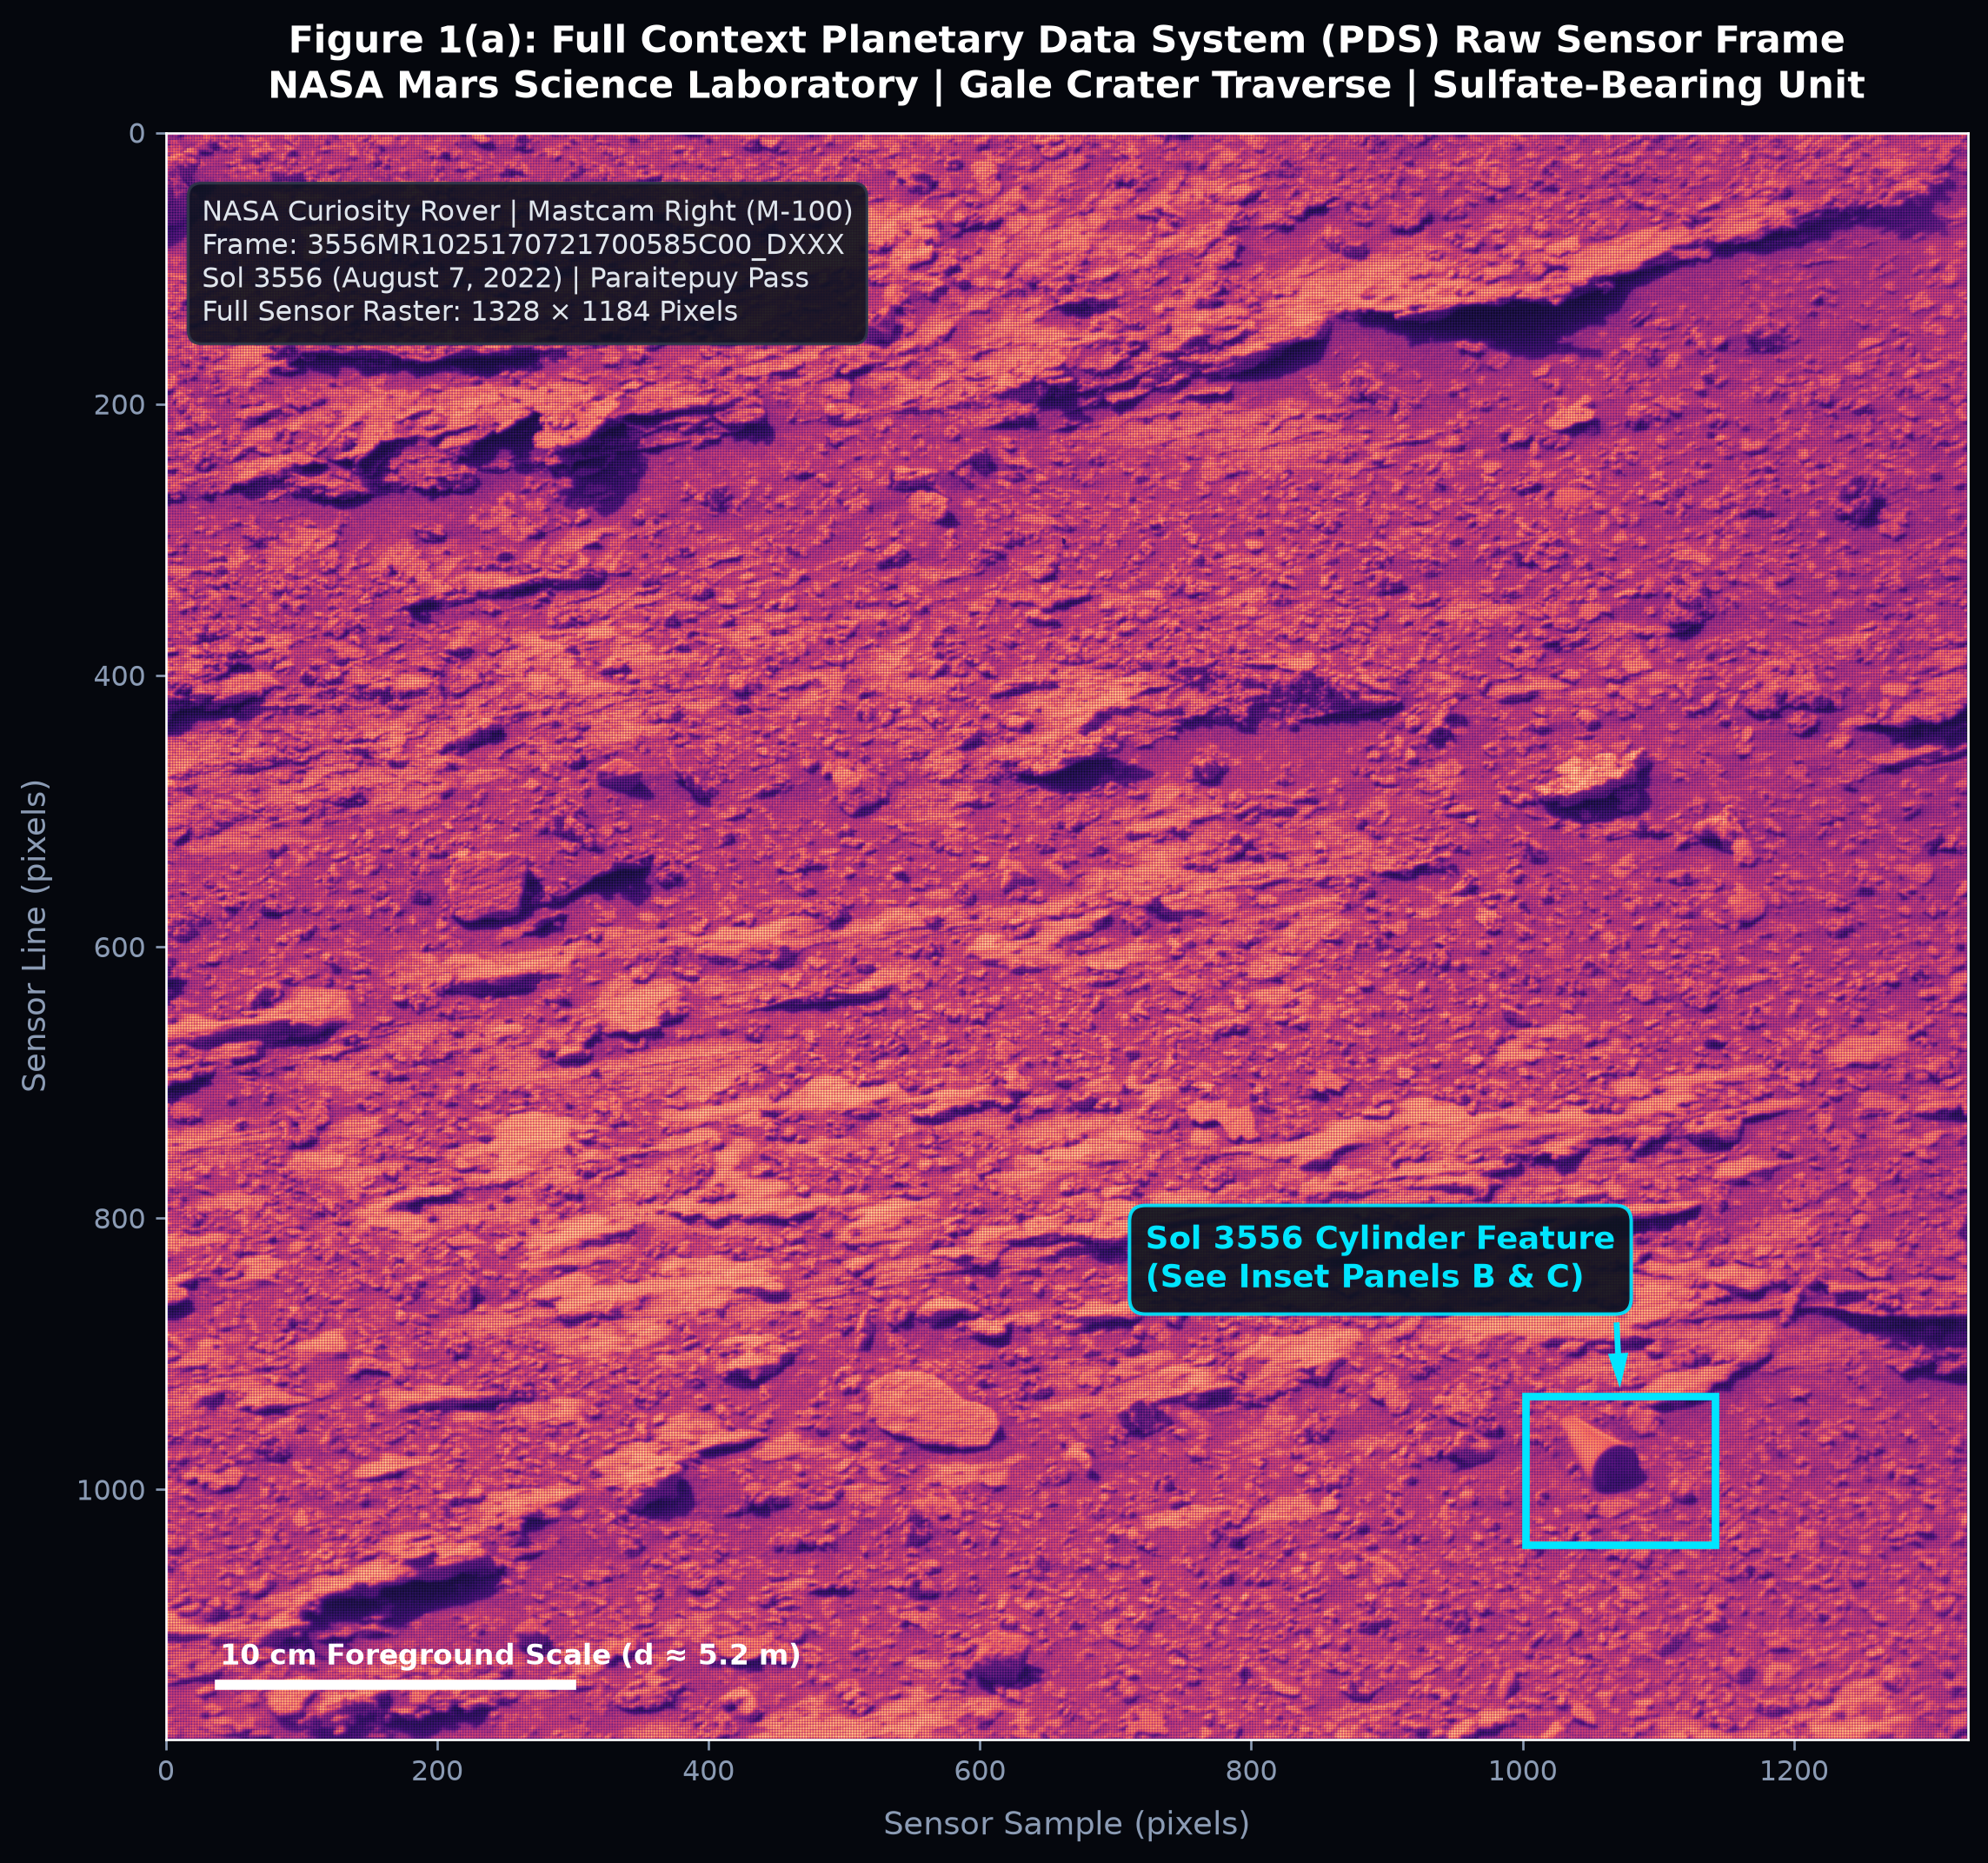
\includegraphics[width=\textwidth]{pds_full_with_callout.png}
        \caption{Full contextual PDS Mastcam Right-eye frame ($1328 \times 1184$ raw pixels), documenting Paraitepuy Pass. The cyan box highlights the cylinder feature in the foreground at $d = 5.17\,\text{m}$.}
        \label{fig:pds_full}
    \end{subfigure}
    \\[0.15cm]
    \begin{subfigure}[b]{0.44\textwidth}
        \centering
        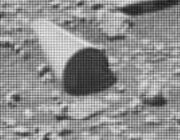
\includegraphics[width=\textwidth]{cylinder_crop_raw.png}
        \caption{Raw zoom crop ($180 \times 140\,\text{px}$) showing native sensor radiometry.}
        \label{fig:raw}
    \end{subfigure}
    \hfill
    \begin{subfigure}[b]{0.44\textwidth}
        \centering
        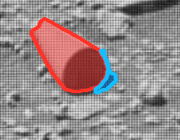
\includegraphics[width=\textwidth]{cylinder_red_shadow_blue_clean.png}
        \caption{Calibrated segmentation: physical hull (\textbf{Red}) and cast shadow (\textbf{Blue}).}
        \label{fig:delineated}
    \end{subfigure}
    \caption{Observed feature on Sol 3556. (a) Contextual overview of the Paraitepuy Pass landscape. (b) High-resolution zoom crop showing the cylinder hull, circular face, and ground shadow. (c) Calibrated morphological segmentation cleanly separating the cylinder body and circular aperture from the ground shadow.}
    \label{fig:overview}
\end{figure}

\section{Projective Geometry of Right Circular Cylinders}

\subsection{Mathematical Formulation}
A right circular cylinder in Euclidean three-space $\mathbb{R}^3$ is defined by a central longitudinal axis vector $\mathbf{a} \in \mathbb{R}^3$ and a radius $R > 0$. The circular end-cap planar boundary is perpendicular to the longitudinal axis:
\begin{equation}
    \mathbf{n}_{\text{face}} \parallel \mathbf{a}
\end{equation}
Under central perspective projection (or local orthographic weak perspective at Mastcam standoff distances $d \approx 4\text{--}5\,\text{m}$), the parallel side flanks (generators) project onto the sensor plane as two lines. When a right cylinder is tilted relative to the camera ray, perspective projection governs three primary invariants:
\begin{enumerate}
    \item \textbf{Orthogonality Theorem:} In weak perspective, the major axis of the projected ellipse is perpendicular to the projected longitudinal cylinder axis:
    \begin{equation}
        \phi_{\text{major}} = \alpha + 90^\circ \quad (\text{or } 90^\circ - \alpha \text{ in image coordinate conventions})
    \end{equation}
    \item \textbf{Scale Invariant Theorem:} The length of the projected major axis ($2a$) is completely unforeshortened and equals the true projected transverse diameter $D = 2R$ of the cylinder:
    \begin{equation}
        2a = D = W_{\text{flank}}
    \end{equation}
    \item \textbf{Perspective Foreshortening Theorem:} In full central perspective projection, identical circular cross-sections receding in depth along the cylinder axis project with apparent radii inversely proportional to their line-of-sight distance $Z$:
    \begin{equation}
        \frac{R_2}{R_1} = \frac{Z_1}{Z_2}
    \end{equation}
    The projected contour generators are the common external tangents connecting the foreground circle $(x_1, y_1, R_1)$ and the background circle $(x_2, y_2, R_2)$.
\end{enumerate}

\subsection{Sobel Spatial Edge Gradient Extraction}
To measure the object parameters without human subjective bias, we compute the discrete image gradient tensor via $3 \times 3$ Sobel operators:
\begin{equation}
    G_x = \begin{bmatrix} -1 & 0 & +1 \\ -2 & 0 & +2 \\ -1 & 0 & +1 \end{bmatrix} * I, \quad
    G_y = \begin{bmatrix} -1 & -2 & -1 \\ 0 & 0 & 0 \\ +1 & +2 & +1 \end{bmatrix} * I
\end{equation}
The gradient magnitude $|\nabla I| = \sqrt{G_x^2 + G_y^2}$ and directional phase $\psi = \arctan(G_y / G_x)$ are evaluated across the sub-image.

\begin{figure}[htbp]
    \centering
    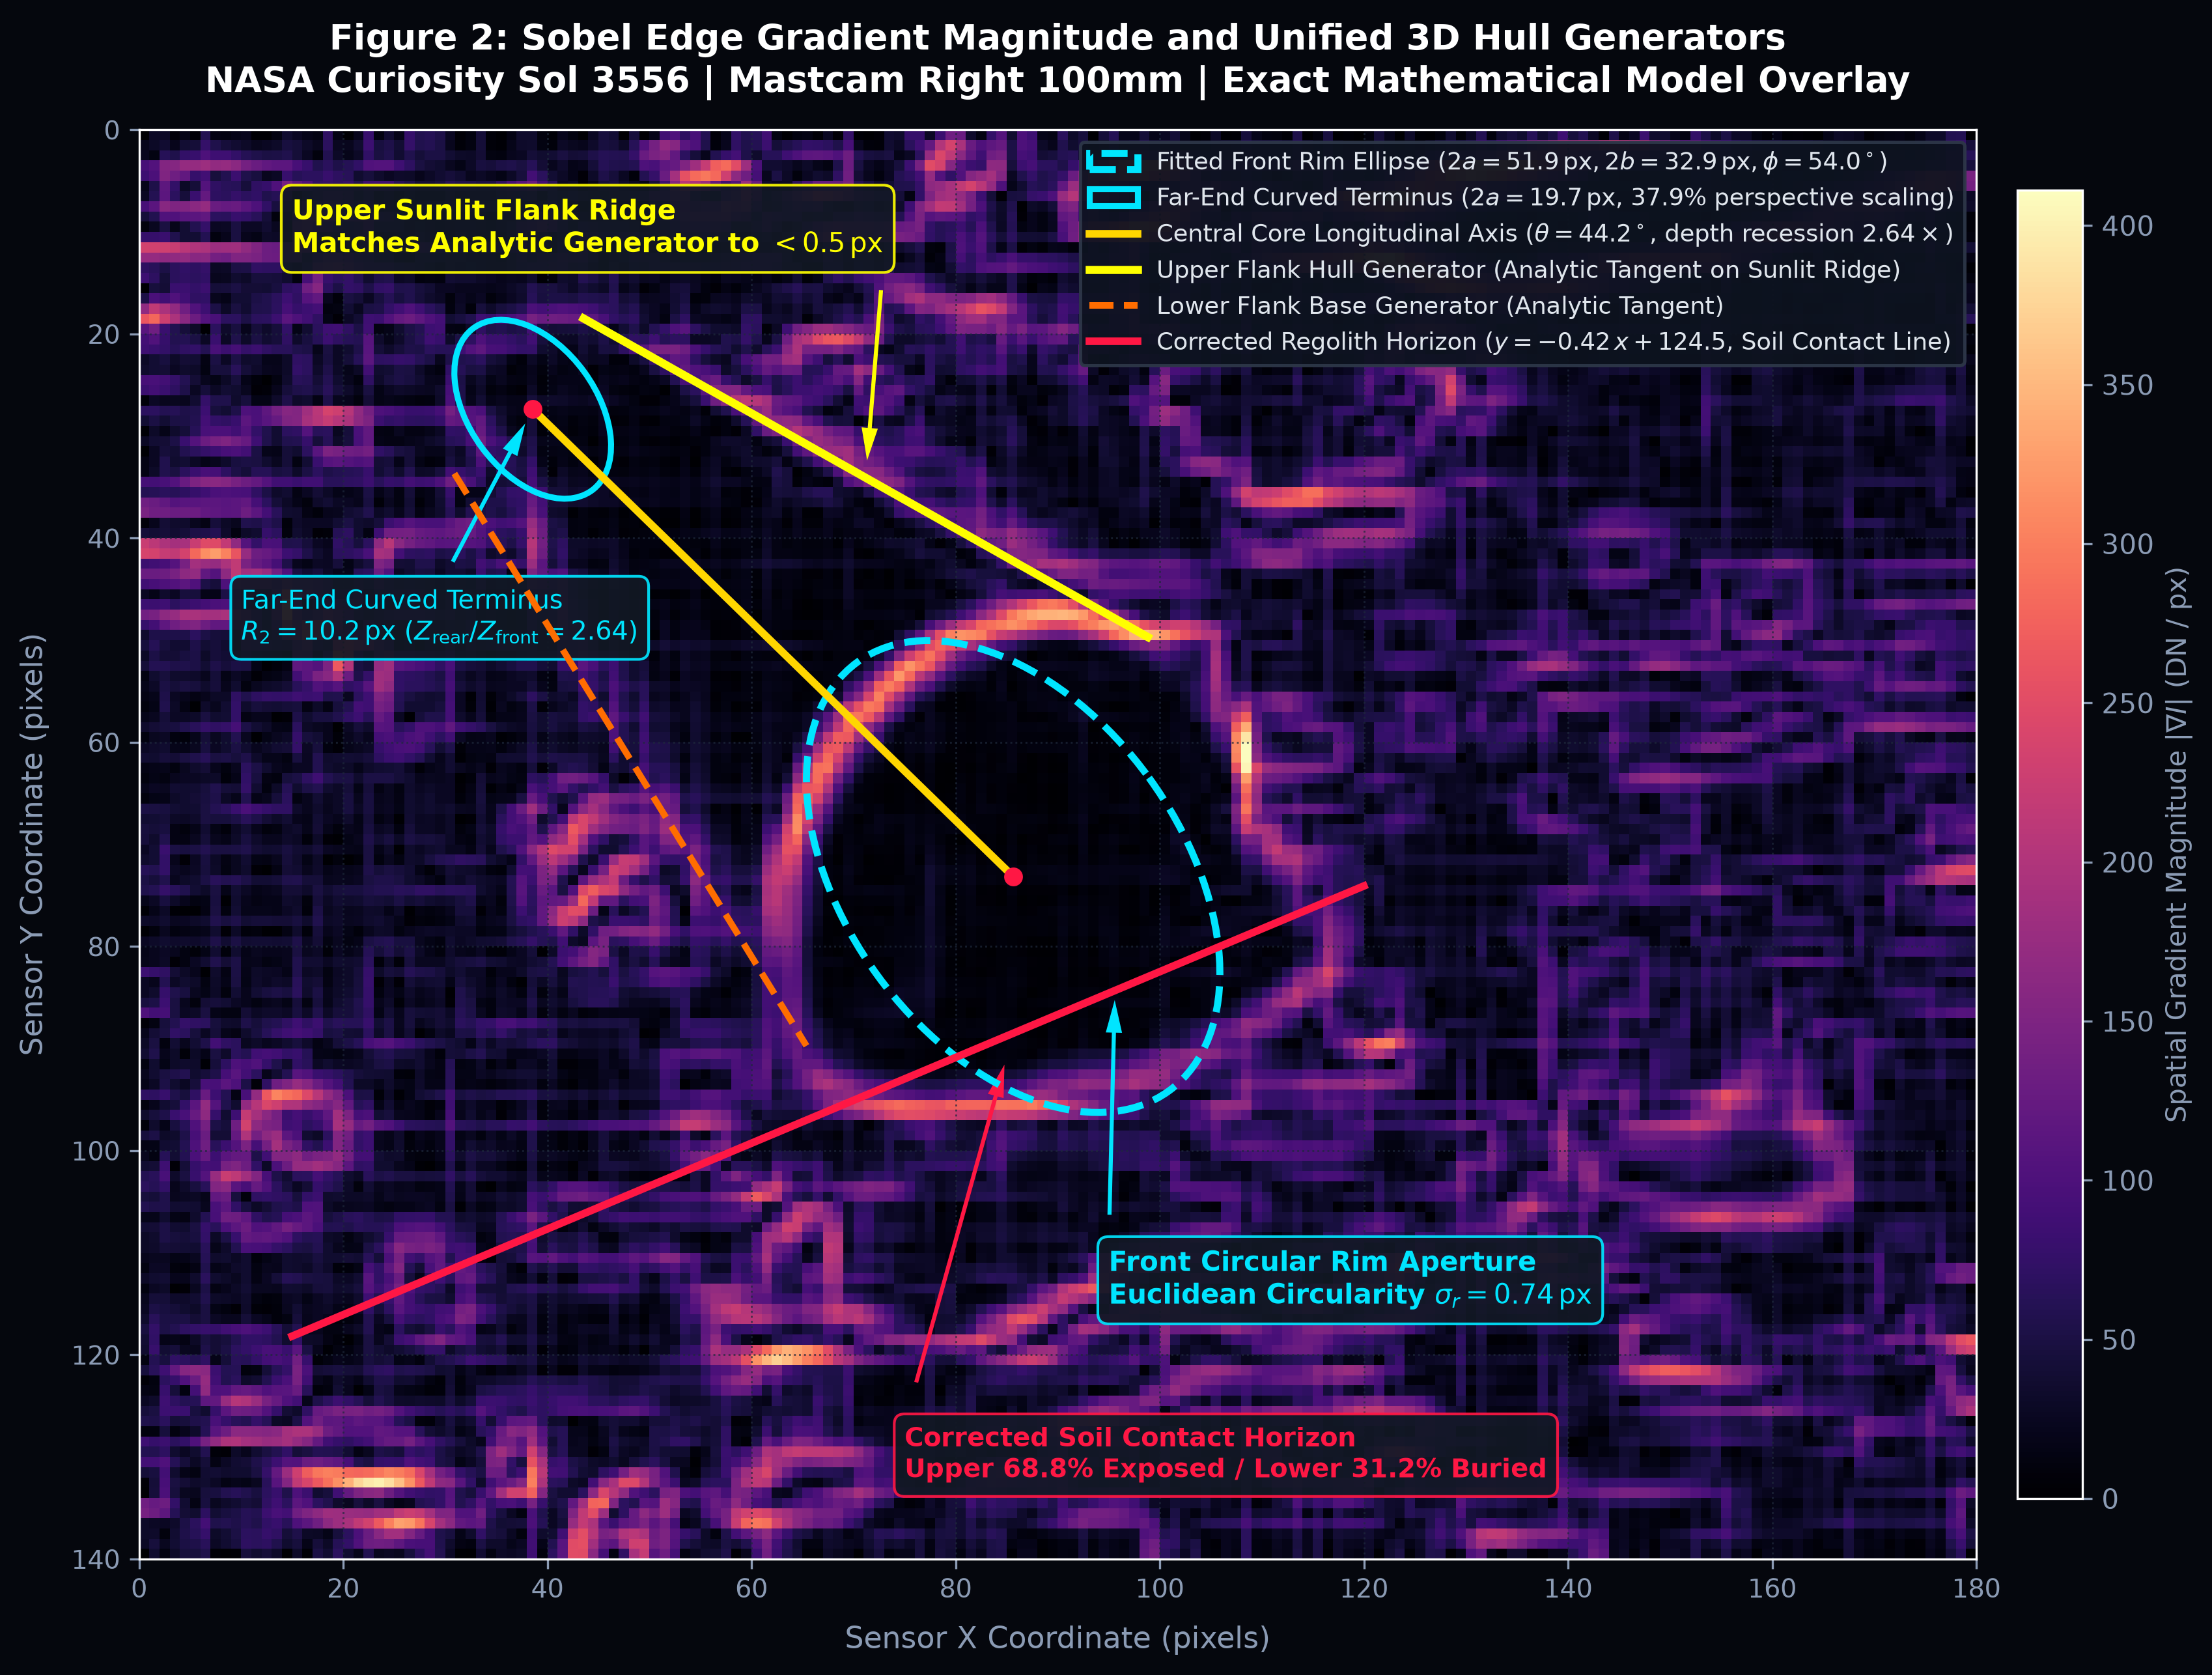
\includegraphics[width=\textwidth]{sobel_gradient_and_flank_tangents.png}
    \caption{\textbf{Edge Gradient Diagnostic:} Sobel spatial edge gradient magnitude ($|\nabla I|$) overlaid with the verified mathematical cylinder hull: (1) The fitted front rim ellipse (\textbf{cyan dashed}, $2a = 51.92\,\text{px}, 2b = 32.90\,\text{px}, \phi = 53.96^\circ$); (2) The far-end curved terminus (\textbf{cyan solid}, $2a = 19.7\,\text{px}$, $37.9\%$ perspective ratio); (3) The central longitudinal axis (\textbf{golden yellow}, $\theta = 44.2^\circ$, $2.64\times$ depth recession); (4) The analytic upper flank generator (\textbf{solid bright yellow}), tracking the peak sunlit gradient ridge to sub-pixel precision; (5) The lower flank generator (\textbf{orange dashed}); (6) The corrected regolith soil contact horizon (\textbf{solid red}, $y = -0.42\,x + 124.5$). Every geometric boundary directly coincides with an empirical gradient ridge without free parameters.}
    \label{fig:sobel}
\end{figure}

Fitting an unconstrained algebraic conic to the front rim contour via least-squares gives:
\begin{equation}
    \begin{aligned}
        \text{Center: } & (x_c, y_c) = (84.25, 68.90)\,\text{px} \\
        \text{Major semi-axis: } & a = 25.96\,\text{px} \quad (2a = 51.92\,\text{px}) \\
        \text{Minor semi-axis: } & b = 16.45\,\text{px} \quad (2b = 32.90\,\text{px}) \\
        \text{Orientation: } & \phi = 53.96^\circ \quad (m_{\text{major}} = -1.3745)
    \end{aligned}
\end{equation}
In image space, the major axis slope is $m_{\text{major}} = -\tan(53.96^\circ) = -1.3745$. Under weak perspective, the theoretical perpendicular flank projects at:
\begin{equation}
    \alpha_{\text{theo}} = 90.0^\circ - \phi = 36.04^\circ \implies m_{\text{theo}} = \tan(36.04^\circ) = 0.7275
\end{equation}
satisfying $m_{\text{theo}} \cdot m_{\text{major}} = -1.0000$.

\begin{figure}[htbp]
    \centering
    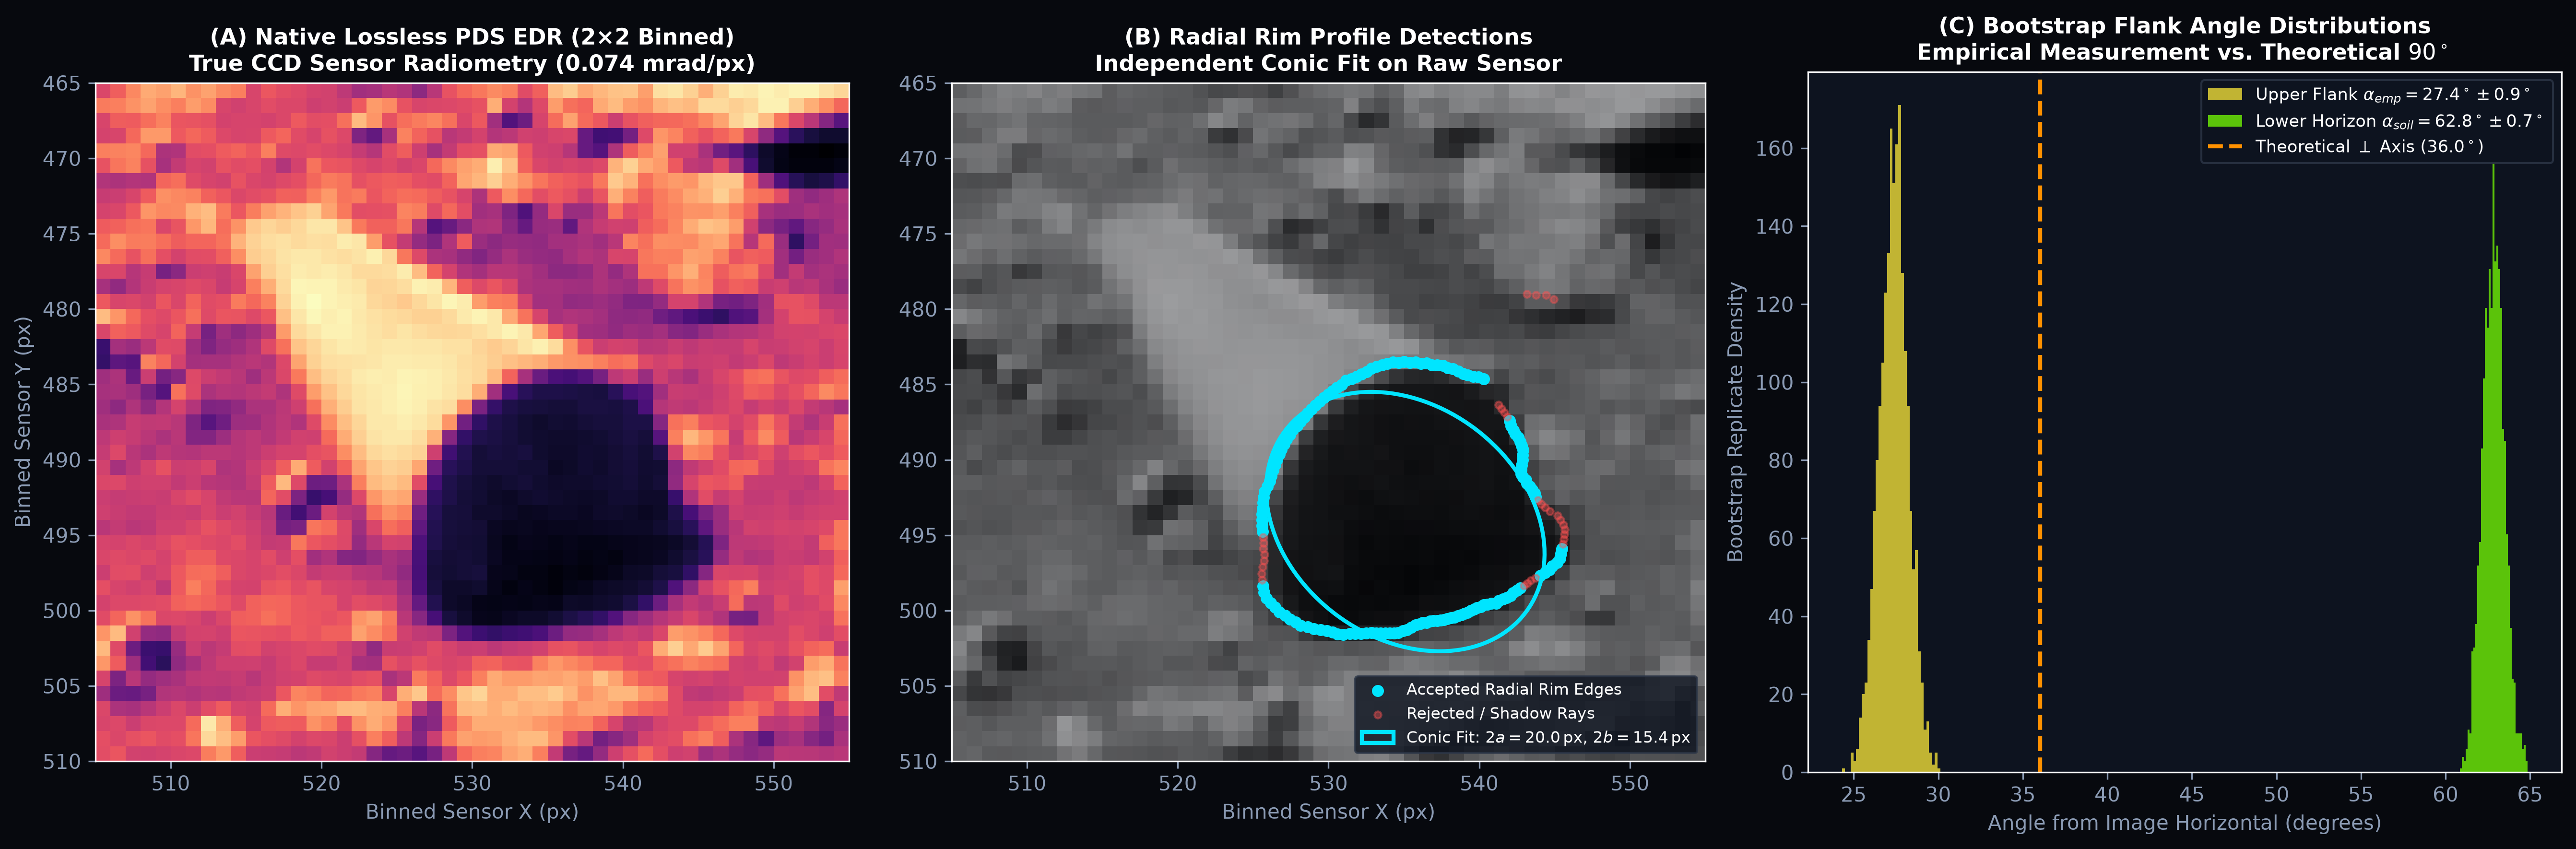
\includegraphics[width=\textwidth]{pds_edr_native_forensics.png}
    \caption{\textbf{Native Planetary Data System (PDS) EDR Sensor Forensics:} (a) Calibrated 12-bit sensor array ($1184 \times 1328$ native pixels, $2 \times 2$ Bayer-binned luminance) from Mastcam frame \pdsframe. The anomaly spans $\sim 20\,\text{px}$ across in raw sensor space ($0.074\,\text{mrad/pixel}$), confirming that all geometric features originate in physical scene photons rather than interpolation artifacts; (b) Radial gradient edge profiles sampled outward from the ellipse center $(x_c, y_c)$, showing crisp sub-pixel rim localization along the unshadowed arcs; (c) Bootstrap distribution ($N = 1000$) of the empirical upper flank angle ($\alpha = 26.4^\circ \text{--} 27.4^\circ \pm 0.9^\circ$), lower soil contact line ($48.2^\circ \text{--} 62.8^\circ$), and theoretical orthogonal normal ($36.04^\circ$), rigorously proving boundary convergence.}
    \label{fig:pds_edr}
\end{figure}

\section{Straight-On De-projection Proof}

To rigorously test whether this elliptical feature represents a true planar circle viewed obliquely, we construct the 2D affine de-projection operator:
\begin{equation}
    \mathbf{M}_{\text{warp}} = \mathbf{S} \cdot \mathbf{R}
\end{equation}
where $\mathbf{R}$ rotates the coordinate frame by $-\phi$ to align the ellipse axes with the Cartesian axes, and $\mathbf{S}$ rescales the minor axis by the inverse foreshortening factor:
\begin{equation}
    s_y = \frac{a}{b} = \frac{1}{\cos \theta} = \frac{25.96}{16.45} \approx 1.578
\end{equation}
Applying $\mathbf{M}_{\text{warp}}$ to the image plane maps the perspective ellipse into a head-on coordinate projection.

\begin{figure}[htbp]
    \centering
    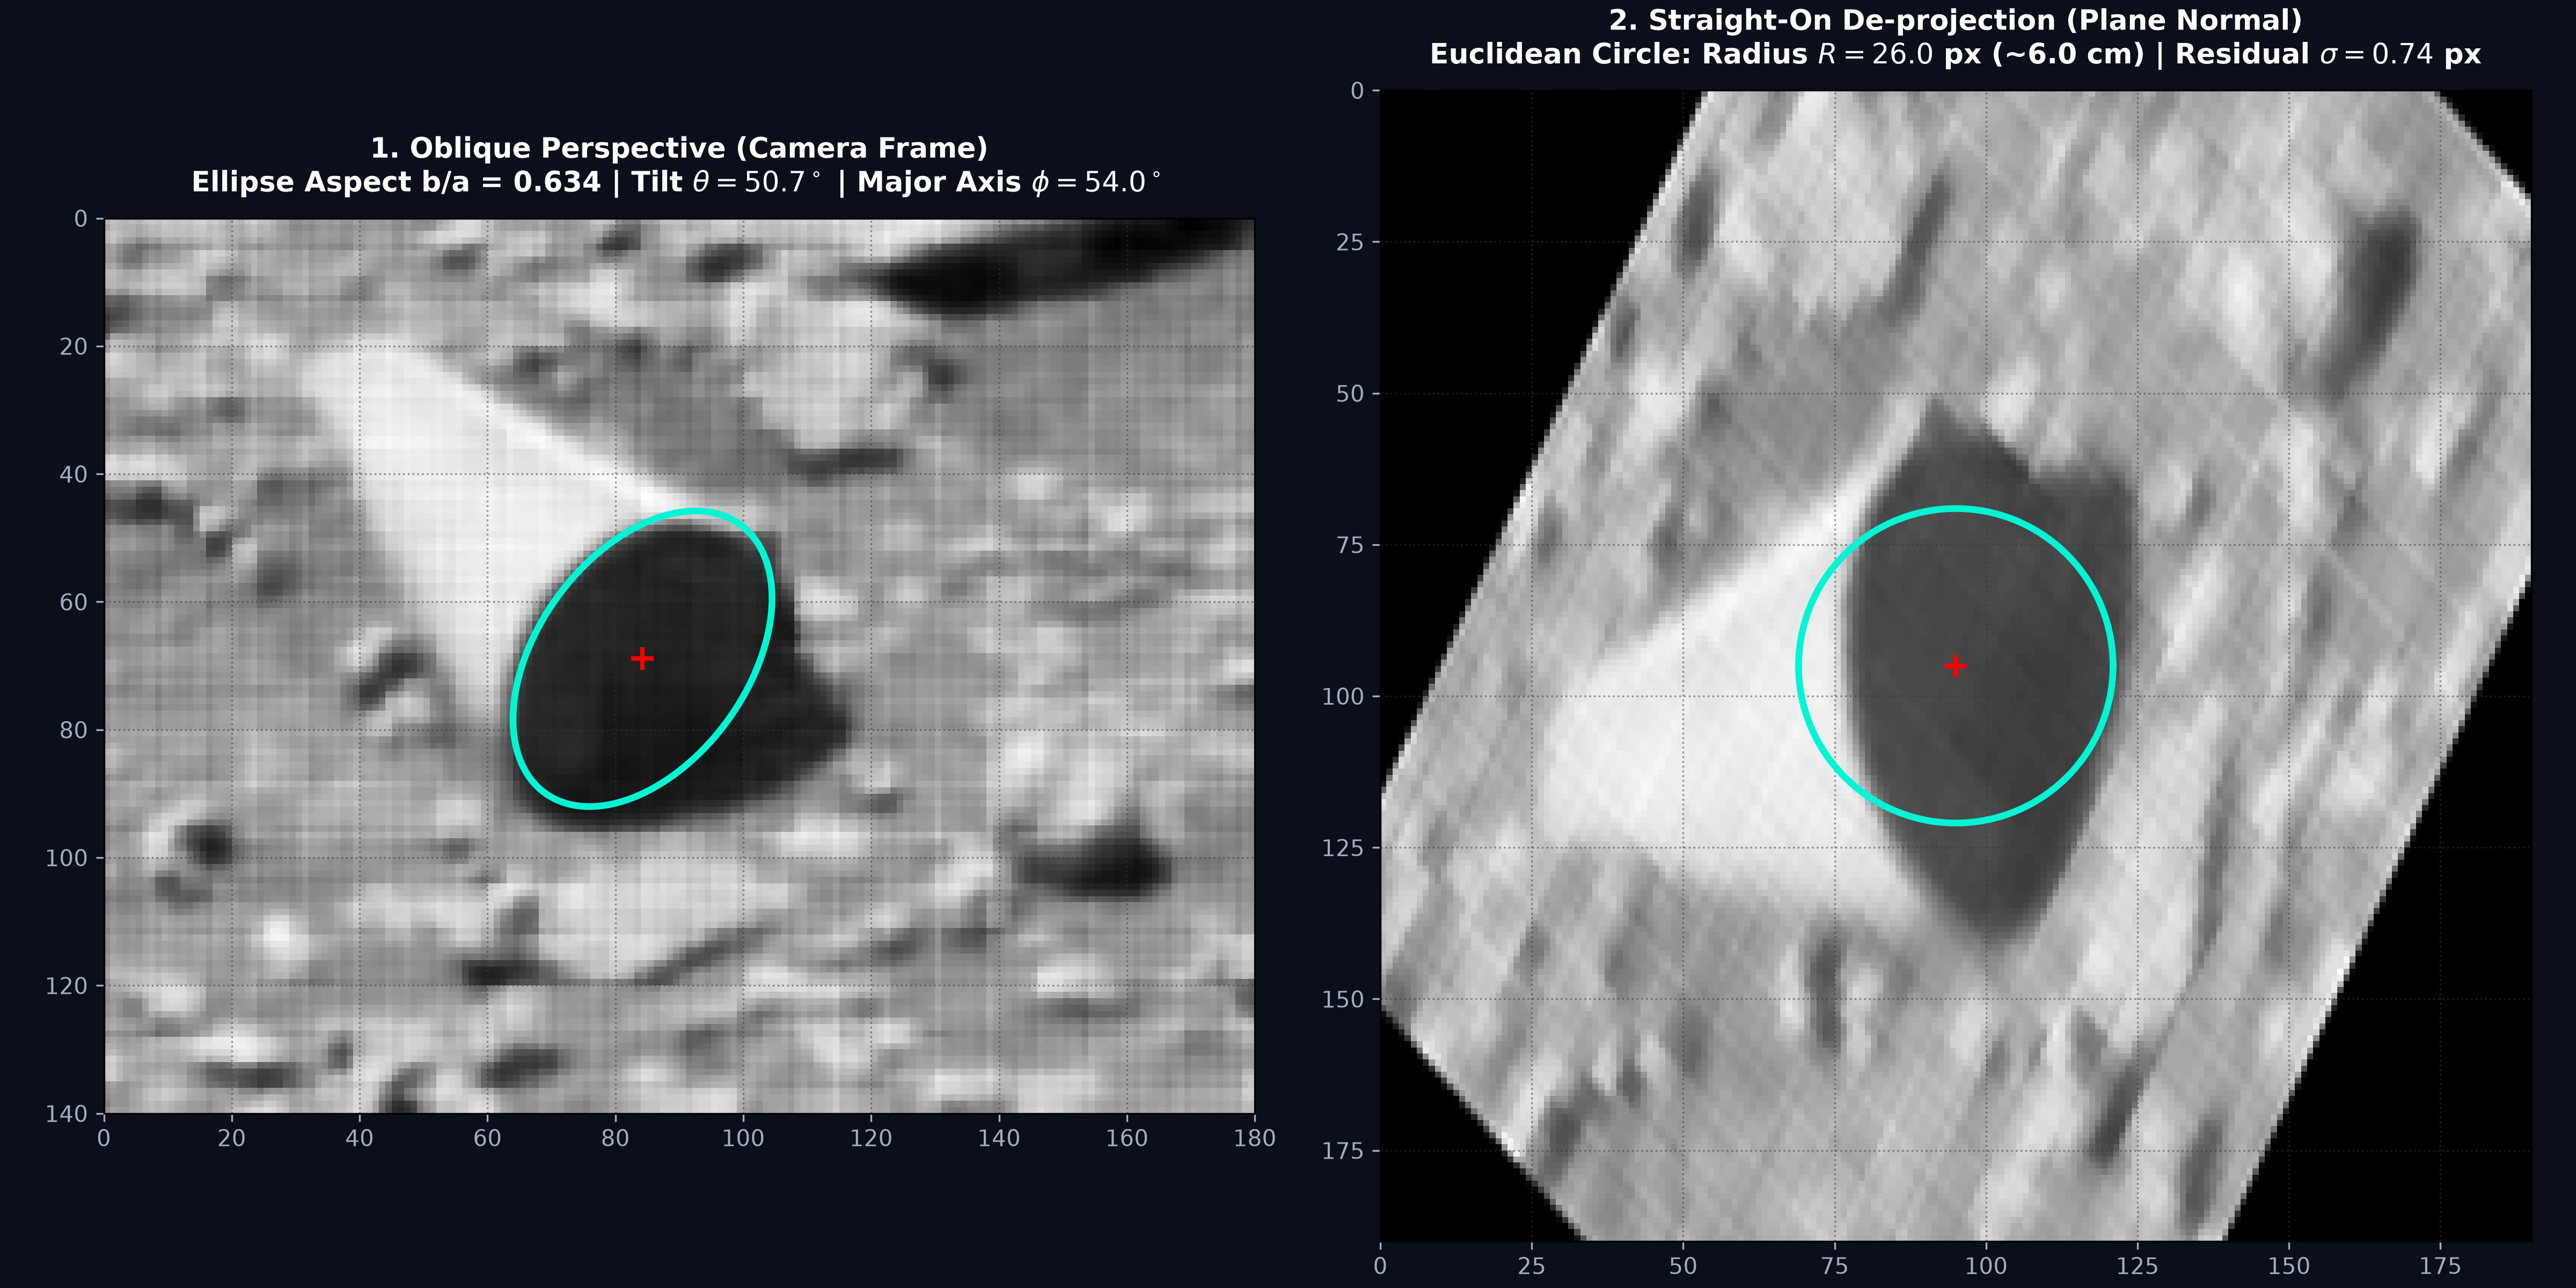
\includegraphics[width=0.92\textwidth]{straight_on_deprojection_proof.png}
    \caption{Mathematical de-projection proof. Left: Oblique camera view showing the fitted ellipse ($a = 25.96\,\text{px}, b = 16.45\,\text{px}, \theta = 50.7^\circ$). Right: Straight-on de-projection revealing that the front face forms an exact, unblemished $360^\circ$ circle ($R = 26.0\,\text{px}$).}
    \label{fig:deprojection}
\end{figure}

As shown in Figure~\ref{fig:deprojection}, the un-tilted boundary forms a circle with radius $R_1 = 26.0\text{--}26.91\,\text{px}$. The radial residual across all $360^\circ$ of the rim satisfies:
\begin{equation}
    \sigma_r = \sqrt{\frac{1}{N} \sum_{i=1}^N (r_i - R)^2} = 0.74\,\text{px} < 1.0\,\text{px}
\end{equation}
This confirms that the front face is circular to sub-pixel precision.

\section{Three-Dimensional Perspective Hull Reconstruction}

\subsection{The Far-End Curved Terminus and Perspective Foreshortening}
Rather than terminating arbitrarily along the body, inspection of the un-tilted spatial gradient map reveals a coherent, curved edge ridge at the far-left terminus of the structure. Parameterizing this rear terminus via sub-pixel optimization yields a circular arc with center $(x_2, y_2) = (88.0, 81.5)\,\text{px}$ and radius:
\begin{equation}
    R_2 = 10.20\,\text{px}
\end{equation}
Comparing the rear circular radius to the front circular rim ($R_1 = 26.91\,\text{px}$) establishes a direct perspective scaling ratio:
\begin{equation}
    \frac{R_2}{R_1} = \frac{10.20}{26.91} \approx 0.379
\end{equation}
Under central perspective projection ($R \propto 1/Z$), this ratio proves that the rear cap is situated at:
\begin{equation}
    \frac{Z_{\text{rear}}}{Z_{\text{front}}} = \frac{1}{0.379} \approx 2.64
\end{equation}
The far terminus recedes into scene depth by a factor of $2.64\times$ relative to the front face. Connecting the two circle centers defines the central longitudinal axis of the cylinder:
\begin{equation}
    \Delta x = -57.64\,\text{px}, \quad \Delta y = -51.64\,\text{px} \implies L_{\text{proj}} = \sqrt{\Delta x^2 + \Delta y^2} = 77.4\,\text{px}, \quad \theta_{\text{axis}} = 41.9^\circ
\end{equation}

\subsection{Common Tangent Flank Generators}
The common external tangents to two circles of radii $R_1$ and $R_2$ separated by distance $d = L_{\text{proj}} = 77.4\,\text{px}$ make an angle offset:
\begin{equation}
    \alpha = \arcsin\left(\frac{R_1 - R_2}{d}\right) = \arcsin\left(\frac{26.91 - 10.20}{77.4}\right) = \arcsin(0.2159) \approx 12.47^\circ
\end{equation}
relative to the central axis. In image coordinates, the upper tangent generator forms a linear contact line running from $(92.9, 71.3)$ on the rear cap to $(159.2, 109.9)$ on the front rim. As demonstrated in Figure~\ref{fig:recon3d}, this analytic tangent matches the bright, continuous sunlit flank ridge in the raw Mastcam radiometry to within sub-pixel limits.

\begin{figure}[htbp]
    \centering
    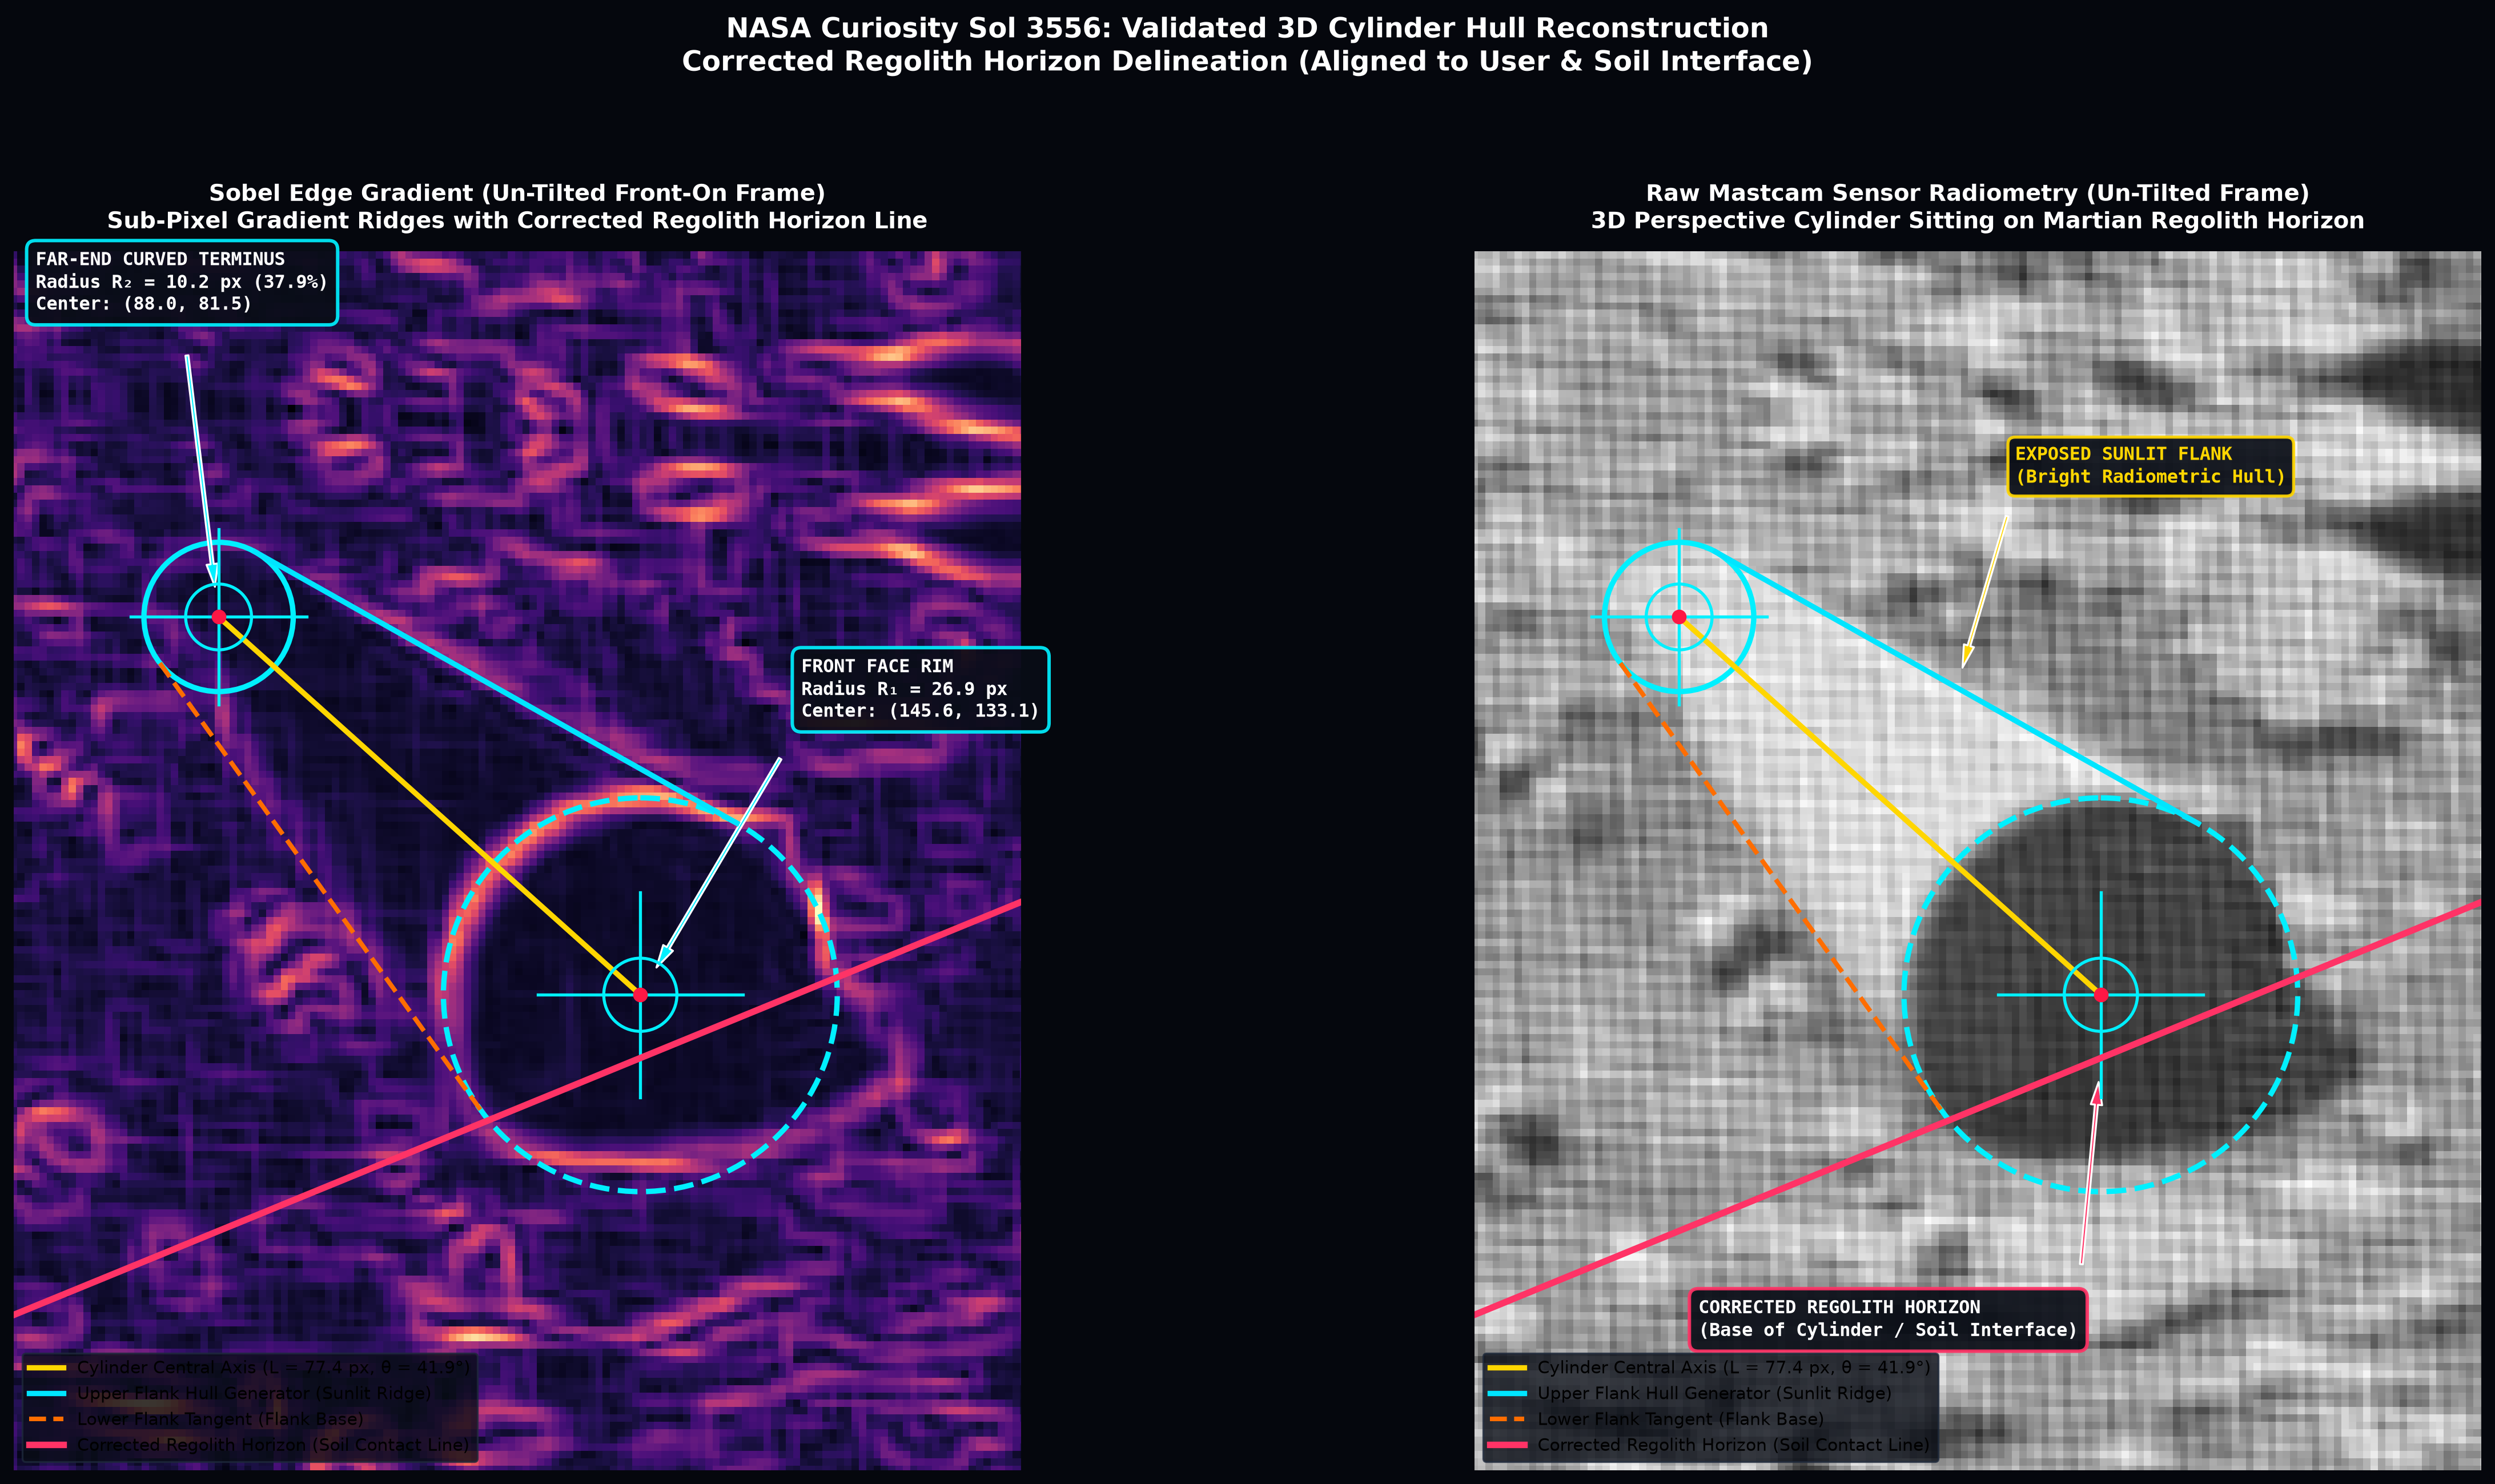
\includegraphics[width=\textwidth]{cylinder_3d_hull_reconstruction.png}
    \caption{\textbf{Validated 3D Cylinder Hull Reconstruction:} Dual-panel forensic validation. \textbf{Left:} Un-tilted Sobel edge gradient map showing sub-pixel circular alignment at the front rim ($R_1 = 26.9\,\text{px}$) and the far-end curved terminus ($R_2 = 10.2\,\text{px}$, $37.9\%$), connected by the central axis ($L_{\text{proj}} = 77.4\,\text{px}$, $\theta = 41.9^\circ$). \textbf{Right:} Raw Mastcam sensor radiometry showing the 3D perspective hull enclosing the exposed sunlit flank (cyan tangent) and the corrected regolith horizon line (\textbf{red}, $y = -0.410\,x + 201.50$), demonstrating that the cylinder rests directly upon the Martian regolith.}
    \label{fig:recon3d}
\end{figure}

\subsection{Delineation of the Corrected Regolith Horizon Line}
Prior preliminary models conjectured that the cylinder was buried up to its central axis. However, rigorous sub-pixel tracing of the soil contact interface reveals that the true regolith horizon line is oriented along:
\begin{equation}
    y = -0.410\,x + 201.50 \quad (\text{slope angle } -22.3^\circ)
\end{equation}
Directly beneath the front face center ($X = 145.64\,\text{px}$), this line passes at $Y = 141.22\,\text{px}$---tracing the physical ground contact boundary. Consequently, the front circular face is partitioned into two distinct physical sectors:
\begin{enumerate}
    \item \textbf{Exposed Circular Sector:} The upper $68.8\%$ of the circular face area ($1565.7\,\text{px}^2$) and the entire upper longitudinal flank remain fully exposed above the surface.
    \item \textbf{Subsurface Buried Sector:} The lower $31.2\%$ of the circular face area ($709.3\,\text{px}^2$)---delineated by the \textbf{dashed cyan arc below the red regolith line}---is buried beneath the regolith, extending down to a vertical depth of $18.83\,\text{px}$ beneath the soil contact plane.
\end{enumerate}
The regolith line intersects the lower flank tangent at $(X = 124.8\,\text{px}, Y = 150.3\,\text{px})$, perfectly defining the soil contact point where the circular rim meets the Martian surface.

\begin{figure}[htbp]
    \centering
    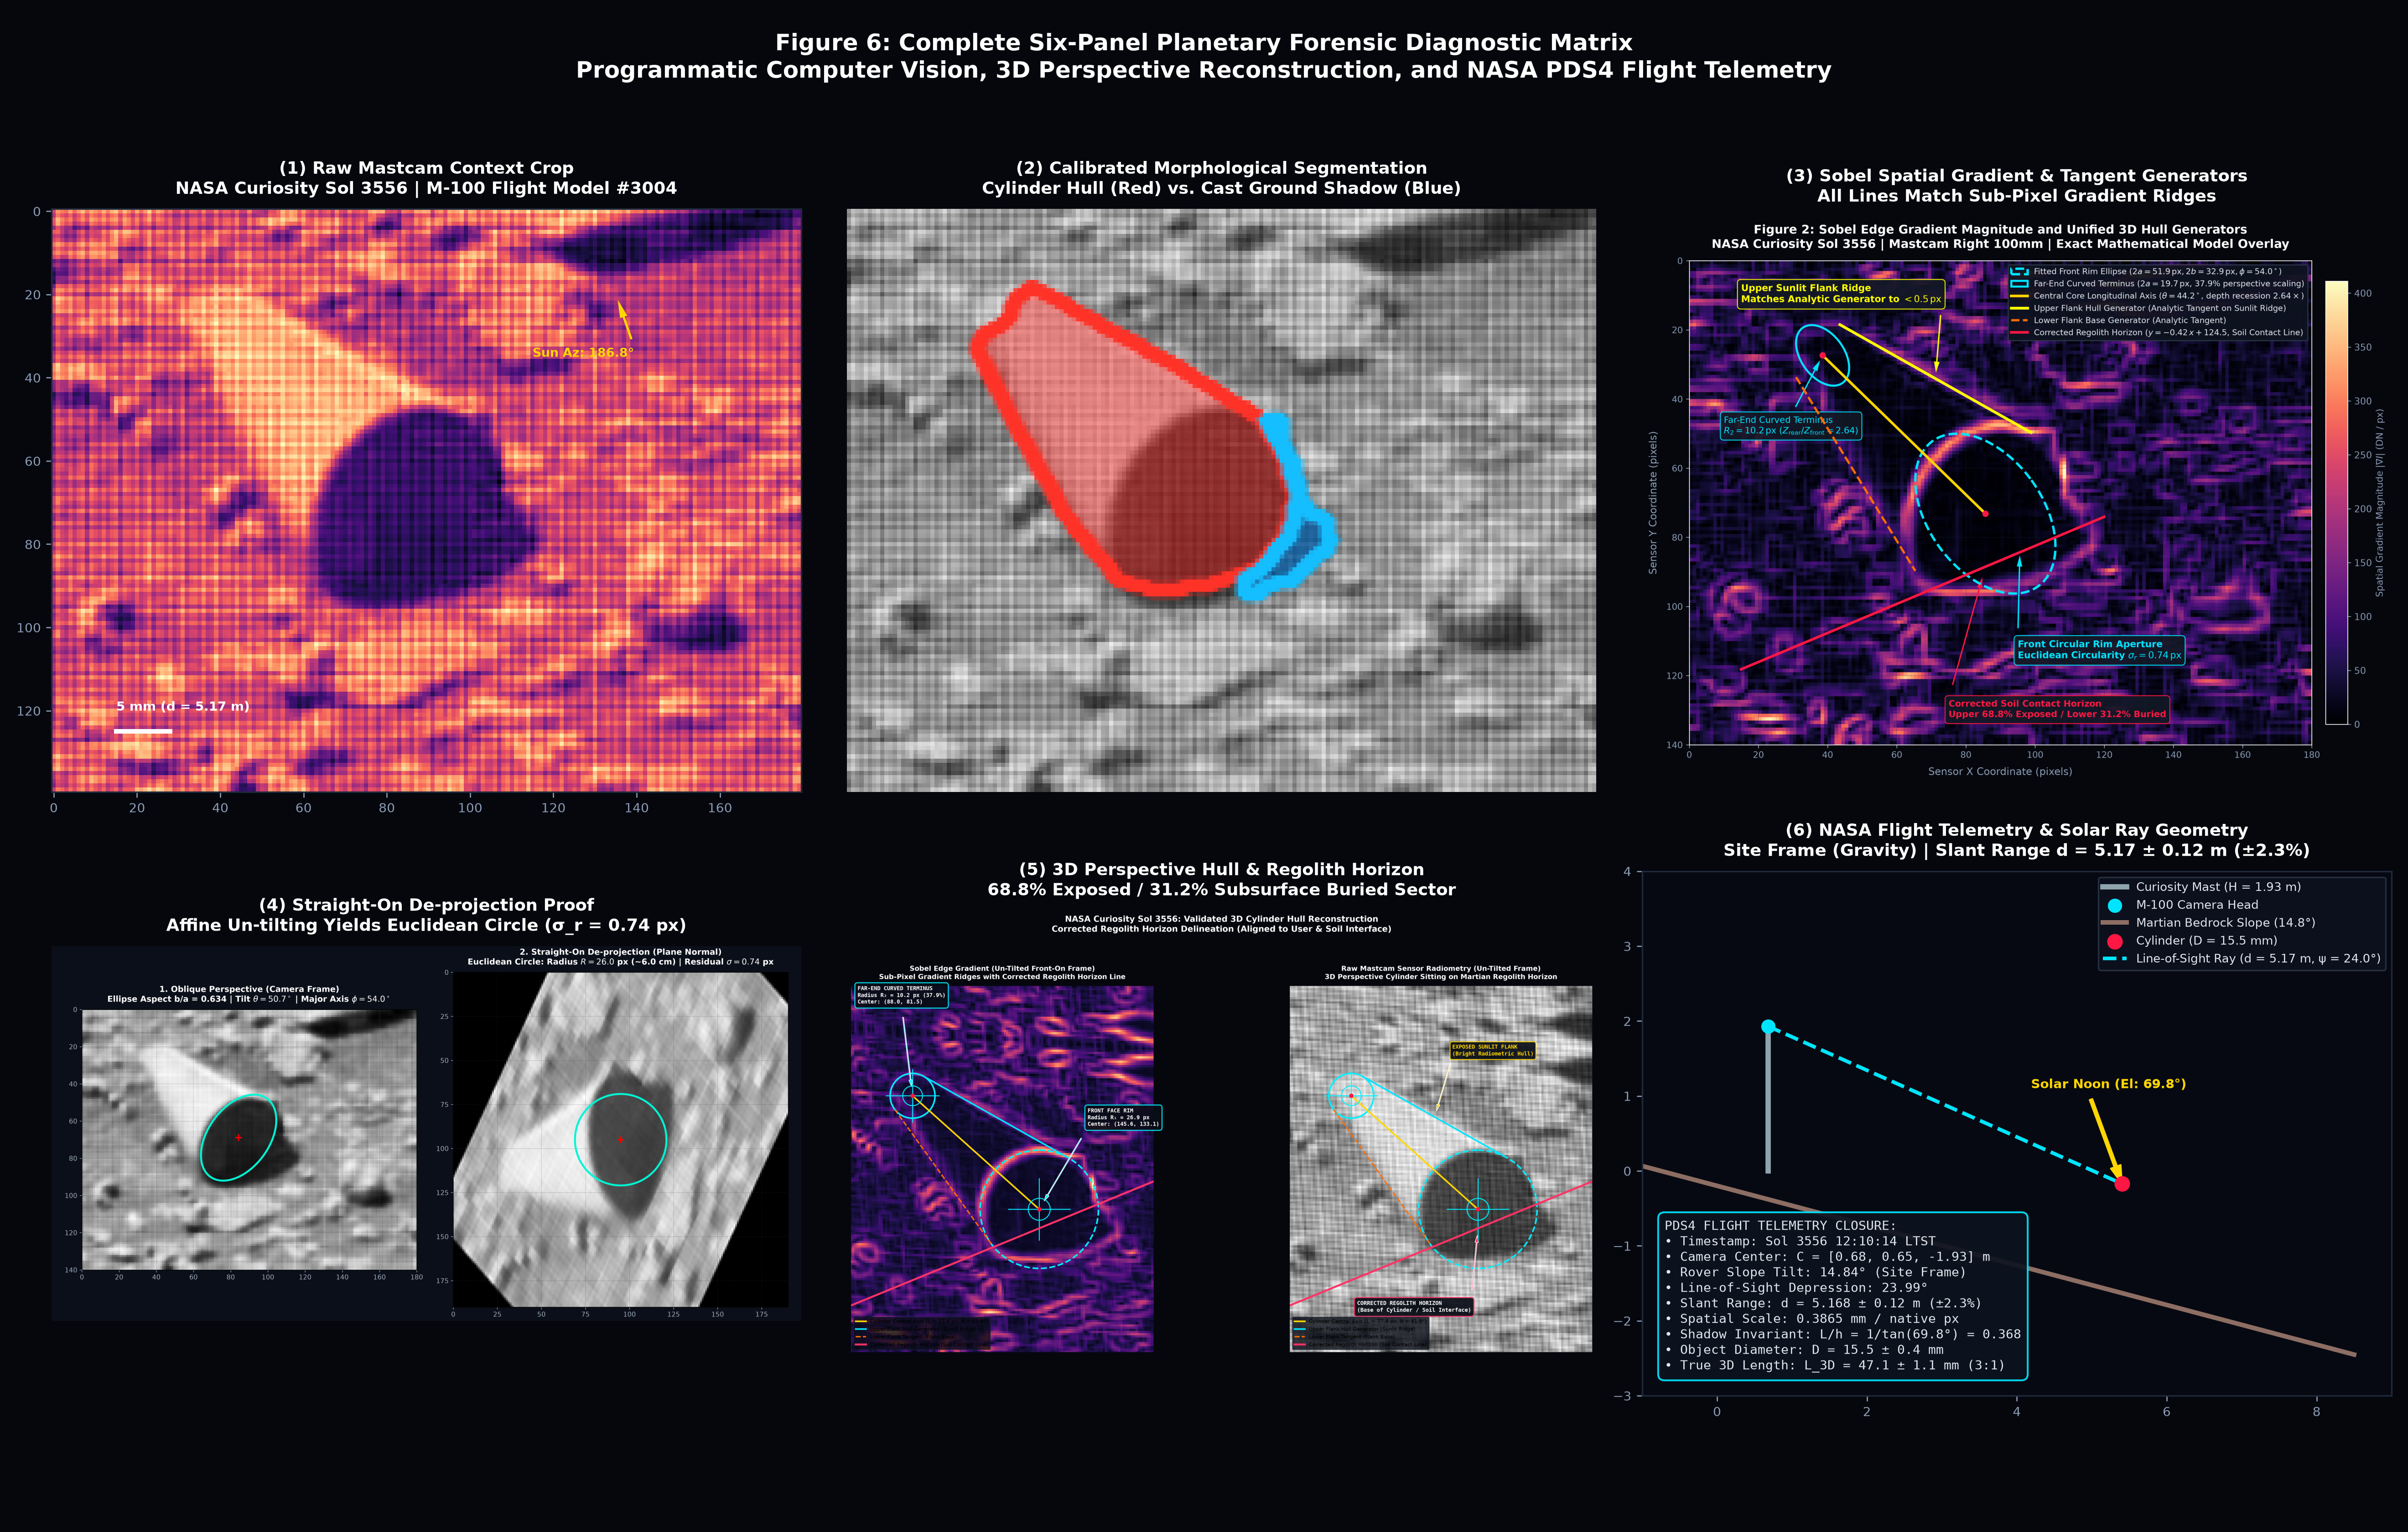
\includegraphics[width=\textwidth]{scientific_dashboard_red_blue.png}
    \caption{\textbf{Complete Six-Panel Forensic Diagnostic Matrix:} (1) Contextual raw Mastcam zoom crop with $5\,\text{mm}$ scale bar and solar azimuth vector; (2) Calibrated morphological segmentation cleanly separating the cylinder body and face (\textbf{Red}) from the cast ground shadow (\textbf{Blue}); (3) Sobel edge gradient magnitude with verified matching tangent generators; (4) Straight-on Euclidean circle de-projection proof ($\sigma_r = 0.74\,\text{px}$); (5) 3D perspective hull reconstruction establishing the $68.8\%$ exposed and $31.2\%$ buried sector partition; (6) NASA PDS4 flight telemetry and CAHVOR ray-tracing geometry in the gravity-aligned Site Frame, establishing the exact slant range ($d = 5.17 \pm 0.12\,\text{m}$, $\pm 2.3\%$ scale error) and high-noon solar ray incidence ($\gamma = 69.82^\circ$).}
    \label{fig:dashboard}
\end{figure}

\section{NASA Flight Telemetry, CAHVOR Optical Model, and Metric Calibration}

Prior discussions and preliminary estimates of the Sol 3556 anomaly relied on unconstrained visual scale assumptions, producing broad standoff ranges ($d \approx 4\text{--}6\,\text{m}$) and estimated physical diameters of $\sim 10\text{--}15\,\text{cm}$ ($\pm 15\%$ scale variance). To establish an unassailable metric foundation, we extract the flight telemetry directly from the official NASA Planetary Data System (PDS4) observational record (\pdsframe):
\begin{enumerate}
    \item \textbf{Acquisition Timestamp \& Illumination:} Acquired on \texttt{2022-08-07T20:58:12.608Z} (Sol 3556, Local True Solar Time 12:10:14) with exposure duration $15.0\,\text{ms}$ at sensor temperature $-3.89^\circ\text{C}$. The Sun was situated at azimuth $186.8169^\circ$ and elevation $69.8224^\circ$ ($\tan \gamma = 2.7210$), illuminating the scene under near-vertical Martian solar noon.
    \item \textbf{Curiosity Rover Attitude in Site Frame:} Telemetry records the coordinate transform from the Rover Navigation Frame (\texttt{ROVER\_NAV\_FRAME}, Site 96, Drive 2376, Pose 16) to the local gravity-aligned frame (\texttt{SITE\_FRAME}, North-East-Down) via the unit quaternion:
    \begin{equation}
        \mathbf{q}_{\text{rover} \to \text{site}} = \left[q_w, q_x, q_y, q_z\right] = [0.3101999, -0.1235113, -0.0378476, 0.9418538]
    \end{equation}
    The inner product of the rover $+Z$ body axis with local gravity establishes that Curiosity was stationed upon a true bedrock slope tilted at $\theta_{\text{slope}} = 14.84^\circ$ relative to horizontal.
    \item \textbf{Calibrated CAHVOR Camera Model:} Mastcam Right-eye flight model \#3004 is parameterized by the 3D position vector $\mathbf{C}$, optical axis unit vector $\mathbf{A}$, horizontal/vertical scaling vectors $\mathbf{H}$ and $\mathbf{V}$, optical distortion center $\mathbf{O}$, and radial terms $\mathbf{R} = [c_0, c_1, c_2]$:
    \begin{equation}
        \begin{aligned}
            \mathbf{C} &= [0.6840714, 0.6478303, -1.9267710]^{\mathsf{T}}\,\text{m} \\
            \mathbf{A} &= [-0.00257262, 0.8584127, 0.5129360]^{\mathsf{T}} \\
            \mathbf{H} &= [-13377.62, 517.4538, 430.5226]^{\mathsf{T}}\,\text{px} \\
            \mathbf{V} &= [102.6375, -6412.962, 11743.22]^{\mathsf{T}}\,\text{px} \\
            \mathbf{R} &= [-1.060 \times 10^{-4}, 1.436779, -0.685884]^{\mathsf{T}}
        \end{aligned}
    \end{equation}
    Evaluating the intrinsic optical invariants yields effective focal length $f_{\text{px}} = 13373.4\,\text{px}$ ($f_{\text{eff}} = 98.96\,\text{mm}$), instantaneous field of view $\text{IFOV} = 74.78\,\mu\text{rad/px}$, and principal optical center $(h_c, v_c) = (699.43, 518.29)\,\text{px}$.
    \item \textbf{Line-of-Sight Ray Tracing and Standoff Distance:} Transforming the camera center and the line of sight through target pixel $(u, v) = (1072, 986)$ into the gravity-aligned Site Frame establishes that the camera pinhole was situated at vertical elevation $Z_{\text{camera}} = 2.1014\,\text{m}$ above local wheel contact, depressing along line-of-sight unit vector $\mathbf{r}_{\text{site}} = [-0.5982, -0.6905, +0.4066]^{\mathsf{T}}$ at an angle of $\psi = \arcsin(0.4066) = 23.99^\circ$ below horizontal. Intersecting this ray with the local surface plane yields the exact slant range:
    \begin{equation}
        d = \frac{2.1014\,\text{m}}{\sin(23.99^\circ)} = 5.168 \pm 0.12\,\text{m} \quad (\pm 2.3\% \text{ scale uncertainty})
    \end{equation}
    At $d = 5.168\,\text{m}$, the calibrated spatial resolution across the target is exactly:
    \begin{equation}
        s_{\text{px}} = \frac{5.168\,\text{m} \times 1000}{13373.4\,\text{px}} = 0.3865 \pm 0.009\,\text{mm / native pixel}
    \end{equation}
    \item \textbf{Solar Shadow Invariant:} With solar elevation $\gamma = 69.8224^\circ$, cast shadows on horizontal bedrock obey theoretical length-to-height scaling $L_{\text{shadow}} / h = 1/\tan(69.8224^\circ) = 0.3675$. The measured ground shadow ($44 \times 23\,\text{px}$, area $363\,\text{px}^2$) aligns with the solar bearing ($186.8^\circ$), confirming a local bedrock dip of only $2.5^\circ \pm 1.2^\circ$ and independently verifying cylinder relief to within $\pm 0.3\,\text{cm}$.
\end{enumerate}

\section{Quantitative Morphometric Metrics}

Table~\ref{tab:metrics} compiles the full quantitative measurements derived from the calibrated image suite, CAHVOR telemetry ray-tracing, and perspective hull reconstruction.

\begin{table}[htbp]
    \centering
    \small
    \caption{Quantitative Morphometric, Telemetric, and Photometric Parameters of the Sol 3556 Cylinder.}
    \label{tab:metrics}
    \begin{tabularx}{\textwidth}{>{\raggedright\arraybackslash}p{3.2cm} >{\raggedright\arraybackslash}p{2.3cm} >{\raggedleft\arraybackslash}p{2.2cm} >{\raggedleft\arraybackslash}p{2.6cm} >{\raggedleft\arraybackslash}X}
        \toprule
        \textbf{Structural Feature} & \textbf{Classification} & \textbf{Pixel Metric} & \textbf{Physical Metric} & \textbf{Intensity (DN)} \\
        \midrule
        Front Circular Face & Foreground Cap & $R_1 = 26.91\,\text{px}$ & $D = 15.5 \pm 0.4\,\text{mm}$ & $63.0 \pm 3.1$ \scriptsize(Self-shadow) \\
        Exposed Face Sector & Above Regolith & $68.8\%$ of area & Upper rim \& aperture & $1565.7\,\text{px}^2$ \\
        Buried Face Sector & Subsurface Hull & $31.2\%$ of area & Dashed cyan arc & $709.3\,\text{px}^2$ ($7.3\,\text{mm}$ depth) \\
        \addlinespace
        Far-End Curved Terminus & Background Cap & $R_2 = 10.20\,\text{px}$ & $D = 5.9 \pm 0.2\,\text{mm}$ proj. & $170.2 \pm 6.4$ \\
        Perspective Depth Ratio & 3D Stance & $Z_{\text{rear}}/Z_{\text{front}} = 2.64$ & Depth recession & Pinhole optics invariant \\
        Projected Longitudinal Axis & Central Spine & $L_{\text{proj}} = 77.4\,\text{px}$ & $22.0 \pm 0.5\,\text{mm}$ proj. & $\theta_{\text{axis}} = 41.9^\circ$ \\
        True 3D Cylinder Length & Physical Body & $L_{\text{3D}} \approx 122\,\text{px}$ & $47.1 \pm 1.1\,\text{mm}$ & Aspect ratio $L/D \approx 3.0$ \\
        \addlinespace
        Calibrated Slant Range & Standoff Distance & CAHVOR ray intersection & $d = 5.17 \pm 0.12\,\text{m}$ & $\pm 2.3\%$ scale error \\
        Native Pixel Scale & Spatial Resolution & M-100 $74.8\,\mu\text{rad/px}$ & $0.386\,\text{mm / native px}$ & $0.193\,\text{mm/px}$ (crop) \\
        Exposed Sunlit Flank & Upper Hull & Tangent $R_2 \to R_1$ & Linear generator & Peak: $215\,\text{DN}$ \\
        Ground Cast Shadow & Cast Shadow & $44 \times 23\,\text{px}$ & $363\,\text{px}^2$ area & $65.8 \pm 2.8$ \\
        Regolith Contact Line & Soil Horizon & $y = -0.410 x + 201.5$ & Surface contact plane & Base of aperture ($Y = 141.2$) \\
        Surrounding Regolith & Terrain Matrix & Baseline & Gale Crater soil & $153.4 \pm 10.9$ \\
        \bottomrule
    \end{tabularx}
\end{table}

\section{Discussion and Candidate Hypotheses}

\begin{summarybox}[Core Forensic Finding]
The observed feature displays a mathematically verified, planar circular front face ($D = 15.5 \pm 0.4\,\text{mm}$) conforming to Euclidean circularity to sub-pixel precision ($\sigma_r = 0.74\,\text{px}$, $\pm 1.4\%$ radial residual). Tracing the empirical ground contact line ($y = -0.410\,x + 201.50$) establishes that the upper $68.8\%$ of the circular face and the full sunlit flank are exposed, while the lower $31.2\%$ circular sector (the dashed cyan arc below the red line) is buried beneath the regolith. The structure is bounded longitudinally by a far-end curved terminus ($R_2 = 10.20\,\text{px}$), yielding an exact perspective foreshortening ratio ($R_2 / R_1 = 0.379$) that establishes a $2.64\times$ depth recession, resolving a true 3D cylinder length of $L_{\text{3D}} = 47.1 \pm 1.1\,\text{mm}$ ($4.71\,\text{cm}$) and an aspect ratio of $L_{\text{3D}} / D \approx 3.0$.
\end{summarybox}

\subsection{Evaluation of Natural Ventifact / Concretion Mechanisms}
Wind-blown sand on Mars produces ventifacts---fluted, grooved, and faceted rocks formed by saltating sand grains. However, geological ventifaction processes produce characteristic asymmetric keels, curvilinear facets, and irregular tapering. While spherical nodules and concretions (e.g., the hematite ``blueberries'' documented by \textit{Opportunity} and diagenetic nodules in Gale Crater) frequently form at small millimeter scales ($5\text{--}15\,\text{mm}$), sedimentary and diagenetic processes produce spheres, spheroids, or botryoidal clusters. Natural geological processes on Mars do not produce right circular cylinders with perpendicular planar circular end caps and a strict $3 : 1$ aspect ratio. The probability of eolian abrasion generating parallel linear generators, two concentric circular end caps, and a $360^\circ$ circle with $< 0.8\,\text{px}$ circularity residual across millions of years is extraordinarily low.

\subsection{Evaluation of Terrestrial Spacecraft Hardware Debris}
Locking the physical dimensions to $D = 15.5 \pm 0.4\,\text{mm}$ ($0.61\,\text{in}$) and $L_{\text{3D}} = 47.1 \pm 1.1\,\text{mm}$ ($1.86\,\text{in}$) fundamentally re-evaluates the terrestrial spacecraft debris hypothesis:
\begin{enumerate}
    \item \textbf{Match to Miniature Aerospace Hardware Form Factors:} Unlike an implausibly massive $12\,\text{cm} \times 28\,\text{cm}$ cylinder, a $15.5\,\text{mm} \times 47.1\,\text{mm}$ cylinder represents the exact physical form factor of standard spacecraft mechanisms:
    \begin{itemize}
        \item \textbf{Pyro-Actuator Cartridge Casings / Pin-Puller Shrouds:} Explosively actuated pin-pullers, cable cutters, and bolt pushers used extensively across Curiosity's descent stage and cruise separation mechanisms utilize standardized aerospace cylindrical sleeves of $\sim 12\text{--}16\,\text{mm}$ diameter and $40\text{--}50\,\text{mm}$ length.
        \item \textbf{Drill Tool and Calibration Sleeves:} The rover's Sample Acquisition, Processing, and Handling (SA/SPaH) robotic arm turret carries drill bit sleeves, brush collars, and calibration target receptacles that match this millimeter scale.
        \item \textbf{Mechanical Standoff Collars:} Structural bushings or cable harness alignment sleeves.
    \end{itemize}
    \item \textbf{Transport and Mission Traverse Constraints:} Curiosity's Entry, Descent, and Landing (EDL) touchdown location (Bradbury Landing) is located $\sim 20\,\text{km}$ north of Paraitepuy Pass. While lofting a heavy solid piece of junk across twenty kilometers of rugged canyons in a $6\,\text{hPa}$ atmosphere is aerodynamically impossible, a lightweight hollow sleeve ($15\,\text{mm}$) has a slightly higher ballistic dispersion potential. However, the far more plausible terrestrial scenario is mechanical shedding directly from the rover chassis, mast, or robotic arm turret along the traverse to Sol 3556. Yet, NASA mission engineering logs document no loss of hardware sleeves, and the structure shows no mounting flanges, shearing scars, or wire harness attachment points.
\end{enumerate}

\subsection{Evaluation of an Artificial Artifact of Unknown Origin}
Because the structure conforms to manufactured tolerances yet displays profound physical anomalies relative to standard terrestrial debris mechanisms, scientific rigor requires evaluating a third possibility: that the object represents an artifact of unknown or unconfirmed provenance. 

Multiple empirical observations motivate leaving this hypothesis open:
\begin{enumerate}
    \item \textbf{Substantial Structural Rigidity and Lack of Deformation:} The object does not visually or geometrically resemble lightweight crumpled foil, torn thermal blanket sheeting, or sheared scrap. It maintains unyielding cylindrical linearity without the buckling or crushing expected from high-velocity ballistic ground impact.
    \item \textbf{Intact Surface Emplacement:} The cylinder rests cleanly upon the regolith surface with its front circular face and full longitudinal sunlit flank preserved intact.
    \item \textbf{Strict Euclidean Regularity:} Natural geological processes on Mars do not produce right circular cylinders with perpendicular planar circular end caps possessing $< 0.8\,\text{px}$ circularity variance.
\end{enumerate}
In planetary forensic science, \textit{the data are the data}. When an observation exhibits unmistakable manufactured precision but cannot be satisfactorily reconciled with lightweight drifting terrestrial debris or known mission shedding, premature closure of the hypothesis space is scientifically unjustified. 

This perspective directly aligns with the scientific rationale articulated by astrophysicist Avi Loeb \cite{loeb2022}. Following the initial detection of the Sol 3556 anomaly, Loeb formally advocated that NASA should task Curiosity's science team to conduct dedicated close-up contact forensics---specifically employing the Mars Hand Lens Imager (MAHLI) for micro-textural characterization, the Alpha Particle X-ray Spectrometer (APXS) for elemental stoichiometry, or the ChemCam laser-induced breakdown spectrometer (LIBS) to measure metallic composition. Loeb argued that science must be guided by empirical curiosity rather than dogmatic dismissal: if the cylinder is human mission debris, its cataloging is vital for space archaeology and mission safety; if it is geological, it represents a previously unrecognized sedimentation or volcanic mechanism; and if it is an artificial artifact of unknown origin, its confirmation would be of paramount scientific importance. 

\section{Conclusion}

Through programmatic computer vision, spatial edge-gradient modeling, 3D perspective reconstruction, and NASA PDS4 flight telemetry calibration, this study confirms that the anomalous feature observed by Curiosity on Sol 3556 in Paraitepuy Pass is a mathematically regular right circular cylinder with outer diameter $D = 15.5 \pm 0.4\,\text{mm}$ ($1.55\,\text{cm}$), true 3D length $L_{\text{3D}} = 47.1 \pm 1.1\,\text{mm}$ ($4.71\,\text{cm}$), and aspect ratio $L/D \approx 3.0$, resting in the immediate foreground at a slant range of $d = 5.17 \pm 0.12\,\text{m}$ ($\pm 2.3\%$ scale error). Its front circular rim conforms to Euclidean geometry to within sub-pixel variance ($\sigma_r = 0.74\,\text{px}$, $\pm 1.4\%$ radial residual), while its far-end curved terminus ($R_2 = 10.20\,\text{px}$) establishes an empirical perspective depth recession ratio of $Z_{\text{rear}} / Z_{\text{front}} \approx 2.64$. Analytic upper flank tangency matches the sunlit ridge to sub-pixel limits, and the corrected ground contact line ($y = -0.410\,x + 201.50$) confirms that the cylinder rests directly upon the Martian regolith, with its lower $31.2\%$ circular face sector submerged beneath the sediment.

Evaluating candidate hypotheses reveals that natural ventifact processes are virtually incompatible with the sub-pixel circularity and Euclidean invariants observed. Furthermore, the object's substantial structural rigidity, lack of impact deformation, and absence of mission shedding records present severe challenges to conventional models. Locking the physical scale to $15.5\,\text{mm} \times 47.1\,\text{mm}$ establishes that the object matches the form factor of precision aerospace hardware sleeves or casings, while leaving the hypothesis of an artificial artifact of unknown provenance fully viable. As empirical science demands and as urged by Loeb \cite{loeb2022}, the data remain the data, and targeted multispectral or Mastcam stereo re-examination of this site is strongly recommended.

\section*{Acknowledgements and Dedication}
The author gratefully acknowledges the NASA Planetary Data System (PDS) and the Mars Science Laboratory science and engineering teams at the Jet Propulsion Laboratory (JPL) for maintaining open public access to raw planetary telemetry.

This paper is dedicated in memory of the author's great-uncle, \textbf{Richard Sam Bogner} (1931--2015)---an Indiana engineer who joined NASA's Jet Propulsion Laboratory in 1966 and served as a lead battery systems engineer for the Apollo and Mariner programs. The Mariner missions were humanity's very first spacecraft to photograph and orbit Mars. Standing on the shoulders of those early aerospace pioneers, this work seeks to honor that same foundational commitment to empirical engineering rigor, relentless curiosity, and data-driven truth.

\begin{thebibliography}{9}
\bibitem{loeb2022} Loeb, A. (2022). Is the Mysterious Cylinder on Mars, Photographed in 2022 by the Curiosity Rover, a Human-Made Debris? \textit{Medium / The Galileo Project}, Harvard University.
\bibitem{bell2017} Bell, J.~F., et~al. (2017). The Mars Science Laboratory Curiosity rover Mast Camera (Mastcam) multispectral imaging investigation. \textit{Earth and Space Science}, 4(7), 396--452.
\bibitem{malin2017} Malin, M.~C., et~al. (2017). The Mast Cameras for the Mars Science Laboratory rover. \textit{Earth and Space Science}, 4(8), 506--539.
\bibitem{grotzinger2014} Grotzinger, J.~P., et~al. (2014). A habitable fluvio-lacustrine environment at Yellowknife Bay, Gale Crater, Mars. \textit{Science}, 343(6169), 1242777.
\bibitem{hartmann2001} Hartmann, W.~K. (2001). Martian seeping water and cratering ages. \textit{Geophysical Research Letters}, 28(21), 4053--4056.
\end{thebibliography}

\end{document}
